\chapter{Implementation}
\label{ch:implementation_testing}

\section{Quick Start Deployment (Personal Laptop)}

The Aether Quick Start deployment was conducted in a single virtualized environment on a personal laptop. In this setup, we evaluated the core functionalities of Aether SD-Core and simulated a 5G network using gNBsim under resource-constrained conditions. Our configuration closely followed the Aether OnRamp Quick Start guide (see \cite{onramp_docs}), with modifications to accommodate our specific hardware and network environment as described in Chapter~\ref{ch:methodology}.

\subsection{Deployment Configuration and Results}
\label{subsec:sdcore-gnbsim-results}

This section outlines the key configuration details and presents the corresponding results for the core network (SD-Core) and the gNBsim deployment,  as reported in Figure~\ref{fig:quick-start-deployment-overview}.

\paragraph{Kubernetes Cluster Setup:}  
A one-node Kubernetes cluster was deployed using RKE2 version \texttt{v1.24.17+rke2r1} with a dedicated token (\texttt{purdue-k8s-rke2}) and port (\texttt{9345}). The master and worker node configurations were derived from template files. Verification of the cluster was performed using \texttt{kubectl}, and the following screenshot shows the status of all pods across namespaces.

\begin{figure}[H]
    \centering
    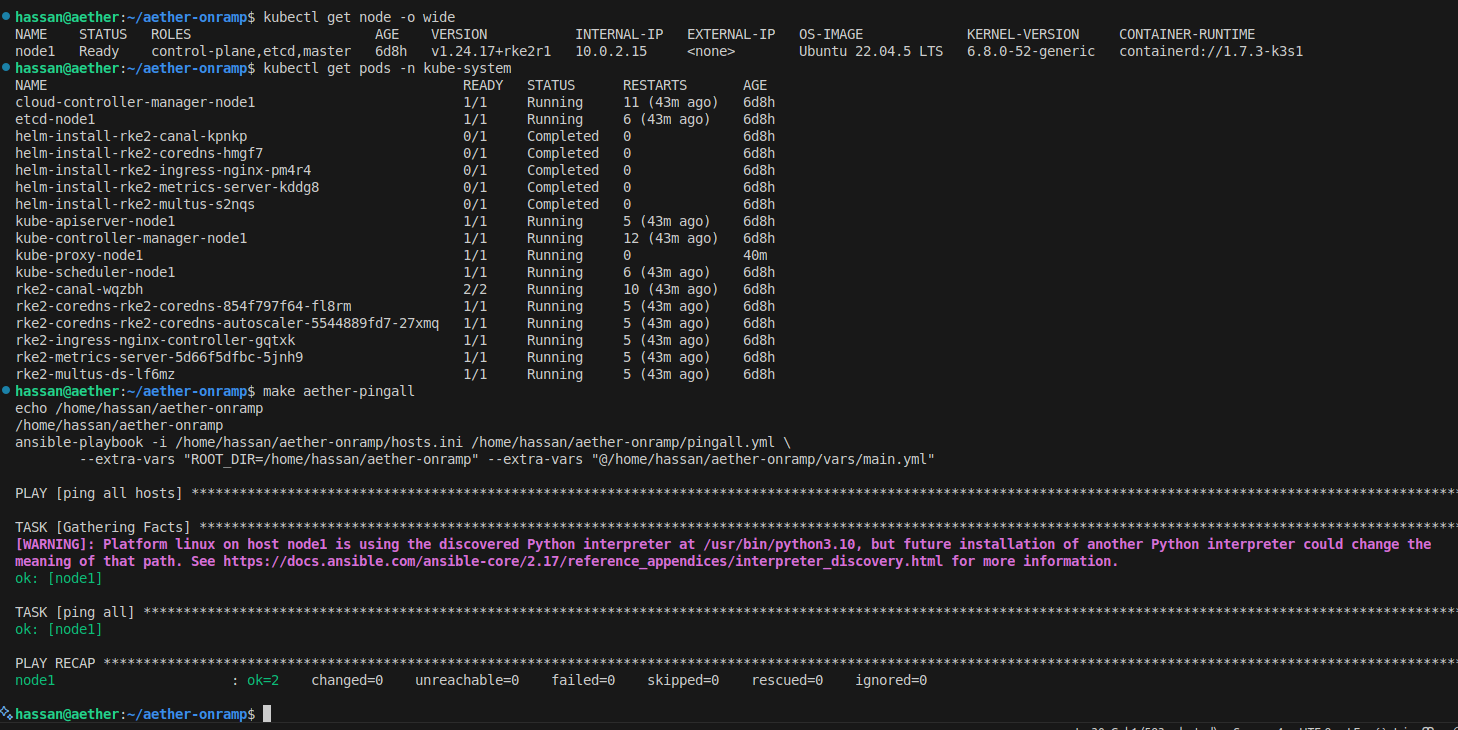
\includegraphics[width=0.8\textwidth]{Hassan_Thesis/images/Single Vm/Deployment&Netwroking/suscessfullk8.png}
    \caption{Kubernetes Cluster Status: Output of \texttt{k8 Successful Deployment}.}
    \label{fig:k8s_cluster_status}
\end{figure}

\paragraph{SD-Core Deployment:}  
The SD-Core was deployed in \emph{standalone} mode, with the data interface set to \texttt{enp0s3}. The configuration was based on the SD-Core values file and explicitly defined the RAN subnet as \texttt{172.20.0.0/16}. The Helm chart \texttt{aether/sd-core} (version \texttt{2.2.2}) was used to deploy the microservices that comprise the 5G core network (including AMF, SMF, UDM, and UPF). The following figure shows the deployment status in the \texttt{aether-5gc} namespace.

\begin{figure}[H]
    \centering
    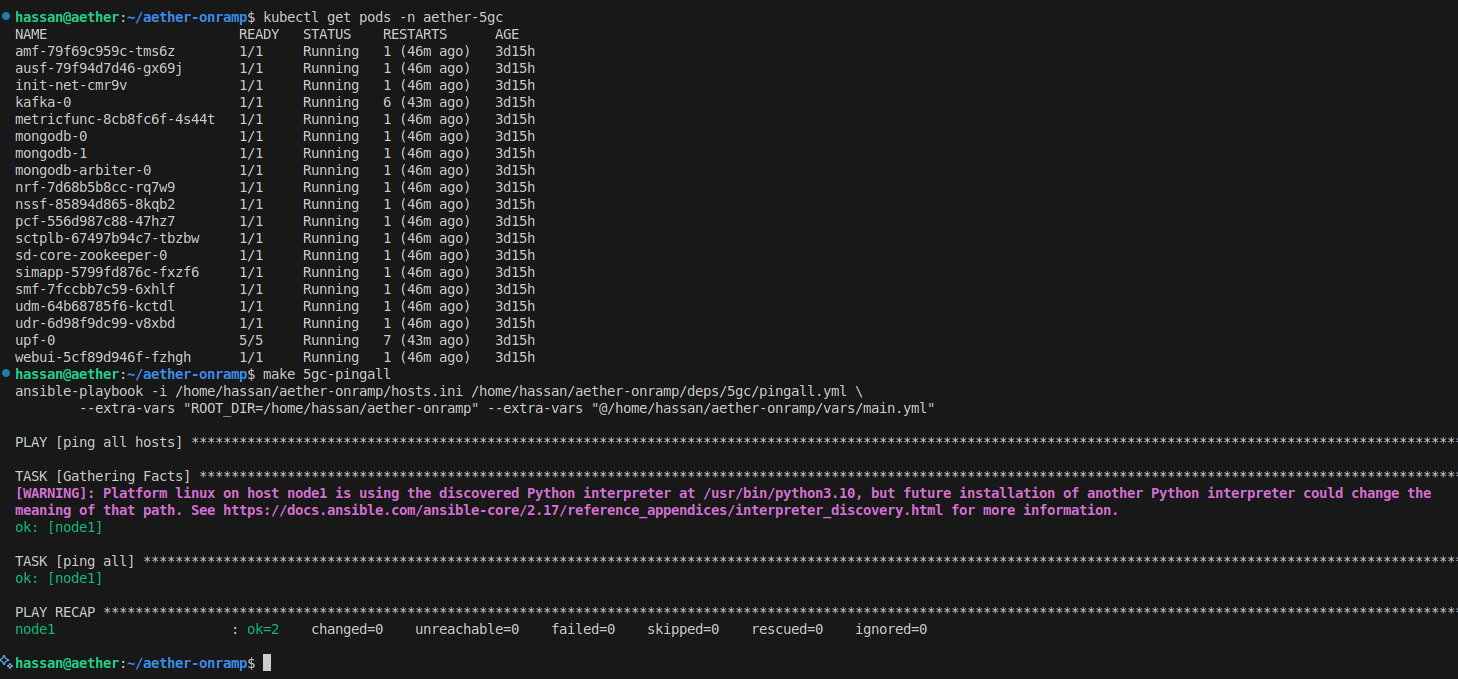
\includegraphics[width=0.8\textwidth]{Hassan_Thesis/images/Single Vm/Deployment&Netwroking/success5gc.png}
    \caption{SD-Core Deployment: Output of \texttt{Successful 5gc Deployment}.}
    \label{fig:sdcore_deployment}
\end{figure}

\paragraph{UPF and AMF Configuration:}  
The UPF was configured with two subnets:
\begin{itemize}
    \item \textbf{Access Subnet:} \texttt{192.168.252.1/24} (default UPF IP: \texttt{192.168.252.3}).
    \item \textbf{Core Subnet:} \texttt{192.168.250.1/24} (default UPF IP: \texttt{192.168.250.3}).
\end{itemize}
An IP pool for user equipment was defined as \texttt{172.250.0.0/16}, and The User Plane Function (UPF) was set to operate in \texttt{af\_packet} mode, a packet I/O method that leverages the standard Linux kernel's socket interface to send and receive raw Ethernet frames. Unlike high-performance modes like DPDK or VPP, \texttt{af\_packet} mode does not require additional kernel modules or drivers, making it easy to deploy and ideal for testbed environments . The AMF was assigned the IP address \texttt{10.0.2.15} to ensure correct signaling with other core components. A screenshot of network connectivity tests or logs confirming these settings is presented below.

\begin{figure}[H]
    \centering
    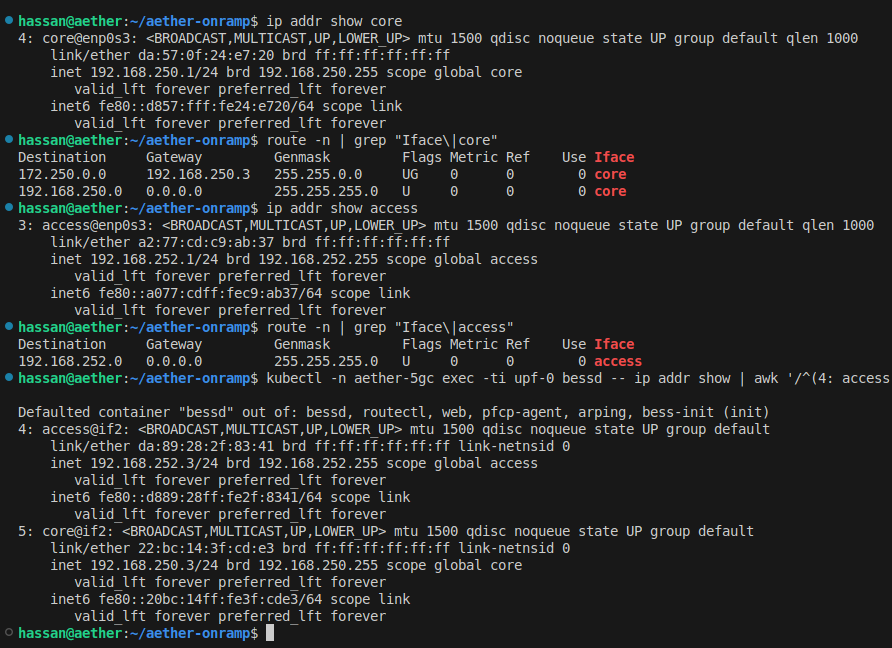
\includegraphics[width=0.8\textwidth]{Hassan_Thesis/images/Single Vm/Deployment&Netwroking/successCor&Access.png}
    \caption{Network Connectivity: Validation of AMF and UPF configurations.}
    \label{fig:amf_upf_status}
\end{figure}

\paragraph{gNBsim Deployment and Testing:}  
The gNBsim container was deployed using the image \texttt{omecproject/5gc-gnbsim:rel-1.6.1}. It was configured with a designated container prefix and attached to a MACVLAN network named \texttt{gnbnet}. The router configuration specified the data interface (\texttt{enp0s3}) and set the MACVLAN subnet prefix as \texttt{172.20}. Following deployment, gNBsim was executed to simulate 5G traffic, including UE registration and PDU session establishment. The test results, extracted from the \texttt{summary.log} file, confirmed that the simulation ran successfully. A representative screenshot of the gNBsim logs is shown below.

\begin{figure}[H]
    \centering
    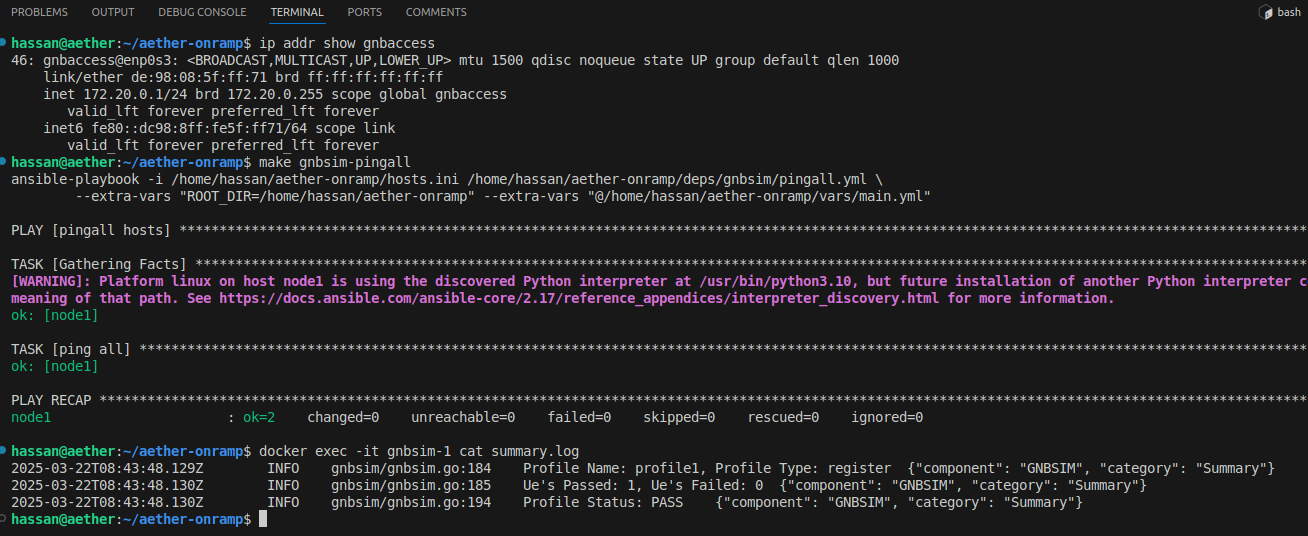
\includegraphics[width=0.8\textwidth]{Hassan_Thesis/images/Single Vm/Deployment&Netwroking/successgNB.png}
    \caption{gNBsim Deployment: Log output showing successful simulation of 5G traffic.}
    \label{fig:gnbsim_status}
\end{figure}

\subsection{Summary of Quick Start Deployment}
\label{subsec:qs-summary}

Our configuration and deployment steps resulted in:
\begin{itemize}
    \item A fully operational Kubernetes cluster with all necessary namespaces and pods active.
    \item Successful deployment of the SD-Core, evidenced by the running state of core network microservices.
    \item Proper configuration and operation of the UPF and AMF, facilitating efficient data and signaling flows.
    \item Effective simulation of 5G traffic via gNBsim, with logs confirming the registration and session establishment processes.
\end{itemize}

These results validate the deployment methodology and serve as a basis for further testing and performance evaluation.

This Quick Start deployment served as a baseline experiment to evaluate the Aether 
platform within a minimal setup. The configuration adhered to the guidelines provided 
by the Aether OnRamp Quick Start documentation, with adjustments made to suit the 
laptop's hardware and network conditions. For a complete listing of the YAML-based 
configuration used in this scenario, see Appendix~\ref{sec:quickstart-config}. The 
insights gained from this deployment---in particular, regarding resource allocation, 
network configuration, and component integration---guided our subsequent, more 
advanced deployment on a high-end lab PC.

\newpage

\section{Full Aether Deployment (Lab PC) Implementation}
\label{sec:full-aether-deployment-impl}

This section details the practical steps undertaken to deploy the full-scale Aether platform on the Lab PC, as outlined in the Methodology chapter. In the following steps, we refer to the hardware specifications (Table~\ref{tab:lab-pc-specs}) and the virtual machine configurations (Tables~\ref{tab:aether-vm} and \ref{tab:ueransim-vm}) that were described earlier. Please refer to Figure~\ref{fig:lab-pc-deployment-overview} for a graphical representation of the deployment environment.

\subsection{VirtualBox Networking Configuration}
\label{subsec:vb-networking-config}

To create a secure and controlled environment for deploying and testing the Aether platform, we configured VirtualBox networking on the Host. Our configuration ensures that:
\begin{itemize}
    \item The \textbf{Aether VM} is assigned a static IP address (\texttt{192.168.56.10}), has full internet access, and is reachable via SSH from the Host machine.
    \item The \textbf{UERANSIM VM} is assigned a static IP (\texttt{192.168.56.20}), is isolated from the internet, and communicates exclusively with the Aether VM.
    \item The Host acts as a router by enabling IP forwarding and configuring NAT, so that internet-bound traffic from the Aether VM is forwarded through the Host’s external interface.
\end{itemize}

\subsection*{1. Host Configuration}
\paragraph{Step 1: Set Up Host-Only Network (vboxnet0)}
On the Host, we used VirtualBox's Host Network Manager to create a network:
\begin{enumerate}
    \item Configure the network with:
    \begin{itemize}
        \item \textbf{IPv4 Address:} \texttt{192.168.56.1}
        \item \textbf{Subnet Mask:} \texttt{255.255.255.0}
        \item \textbf{DHCP Server:} Disabled
        \item \textbf{IPv6:} \texttt{fd00::1/64} (if needed)
    \end{itemize}
\end{enumerate}


\paragraph{IP Forwarding and NAT Configuration on the Host} 
To provide the Aether VM with internet connectivity via the Host, we first enabled IP forwarding and then configured Network Address Translation (NAT) using iptables. IP forwarding was activated to allow the Host to route packets from the internal VirtualBox network (192.168.56.0/24) to its external interface. 
Subsequently, NAT was configured so that all traffic originating from the internal subnet is masqueraded through the Host’s external interface (assumed to be \texttt{wlo1}). This was implemented with the following iptables rule:
\begin{lstlisting}[language=bash]
sudo iptables -t nat -A POSTROUTING -s 192.168.56.0/24 -o wlo1 -j MASQUERADE
\end{lstlisting}

\subsection*{2. Virtual Machine Configuration}

\paragraph{Aether VM.}
For the Aether VM, we configured a single network adapter attached to the host-only network (vboxnet0). A static IP address (192.168.56.10) was assigned to this adapter, and a default route was defined via the Host (192.168.56.1) to enable external connectivity. This setup ensures that the Aether VM remains within a controlled, isolated subnet while still being able to access the internet through the Host. This configuration, as detailed in the Methodology chapter, facilitates remote management and reliable data exchange.

\begin{lstlisting}[language=yaml, caption={Netplan configuration applied to the Aether VM for static routing and DNS setup}]
network:
  version: 2
  ethernets:
    enp0s9:
      dhcp4: false
      addresses:
        - 192.168.56.10/24
      routes:
        - to: 0.0.0.0/0
          via: 192.168.56.1
      nameservers:
        addresses:
          - 8.8.8.8
          - 8.8.4.4
\end{lstlisting}

\paragraph{UERANSIM VM.}
For the UERANSIM VM, a dual-adapter configuration was implemented to provide both operational flexibility and strict experimental isolation. Adapter 1 was connected to the host-only network (vboxnet0) and is used exclusively for simulating UE and gNodeB interactions, ensuring that all experimental traffic remains within a controlled, isolated environment. In parallel, Adapter 2 was configured as a NAT adapter to supply optional internet connectivity for administrative purposes (such as system updates or package installations). However, during the experiments, only the isolated Adapter 1 is utilized, thereby preventing any external network influence on the simulation.

\begin{lstlisting}[language=yaml, caption={Netplan configuration applied to the UERANSIM VM for static routing }]
network:
  version: 2
  ethernets:
    enp0s9:
      dhcp4: false
      addresses:
        - 192.168.56.20/24
      nameservers:
        addresses:
          - 8.8.8.8
          - 8.8.4.4
\end{lstlisting}


\subsection*{Summary}
In summary, our VirtualBox networking configuration achieves the following:
\begin{itemize}
    \item The \textbf{Aether VM} is assigned a static IP (\texttt{192.168.56.10}), has internet access via the Host (IP \texttt{192.168.56.1}), and is reachable via SSH from host.
    \item The \textbf{UERANSIM VM} is assigned a static IP (\texttt{192.168.56.20}) and is isolated from the internet, communicating solely with the Aether VM.
    \item The Host is configured with IP forwarding and NAT, ensuring that the Aether VM’s traffic is correctly routed while keeping the UERANSIM VM isolated.
\end{itemize}

This configuration provides a secure and controlled network environment, which is critical for the deployment and testing of the Aether platform.


\newpage
\subsection{Deployment of Multiple Blueprints (Lab PC)}
\label{subsec:multi-blueprints-deployment}

Building on the foundational Quick Start deployment, we implemented a more advanced Aether platform on a high-performance Lab PC. This deployment leverages multiple blueprints to create a production-like environment in which the SD-Core is deployed in non-standalone mode, integrated with Aether Runtime Operation Control (ROC). This integration enables dynamic management of users, devices, and device groups, and allows for the configuration of UPFs within slices. In addition, the deployment incorporates Aether Monitor, which utilizes Prometheus to collect and store platform and service metrics, and Grafana to visualize these metrics over time.

\subsubsection*{Deployment Architecture and Objectives}
In this deployment:
\begin{itemize}
    \item \textbf{SD-Core with ROC Integration:}  
    The SD-Core is deployed in non-standalone mode, allowing real-time dynamic management of network slices, user profiles, and device groups via ROC. Changes made through the ROC interface (e.g., attaching UPFs to specific slices) are immediately reflected in the SD-Core.
    \item \textbf{Scalable UPF Deployment:}  
    Additional UPF instances are deployed to support multi-path routing and load balancing, accommodating more complex traffic scenarios.
    \item \textbf{UERANSIM Deployment:}  
    The UERANSIM VM simulates realistic 5G user equipment (UE) and gNodeB behavior. It is isolated from direct internet access and communicates exclusively with the Aether VM, ensuring that all simulated traffic is processed within the controlled environment.
    \item \textbf{Aether Monitor:}  
    Monitoring is an integral part of the deployment. Aether leverages Prometheus to collect and store metrics from the core network components and UPFs, while Grafana provides a graphical dashboard for real-time visualization and analysis of these metrics.
\end{itemize}

\subsection*{Key Configuration Details and Process}
The deployment process comprised the following steps:

\begin{enumerate}
    \item \textbf{SD-Core and ROC Integration:}  
    The SD-Core was reconfigured from standalone to non-standalone mode by enabling ROC integration. This adjustment allowed for dynamic management of network slices, user profiles, and device groups. Changes applied via the ROC interface are propagated in real time to the SD-Core.

    \begin{figure}[H]
        \centering
         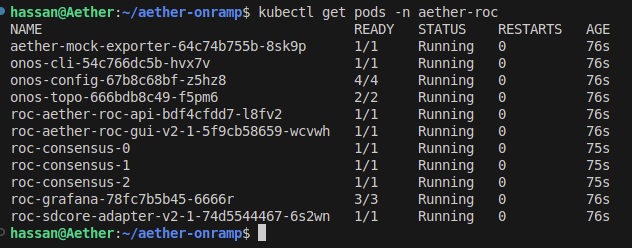
\includegraphics[width=0.8\textwidth]{Hassan_Thesis/images/LAB PC/Deployment&Netwroking/rocinstalledonaethervm.png}        
        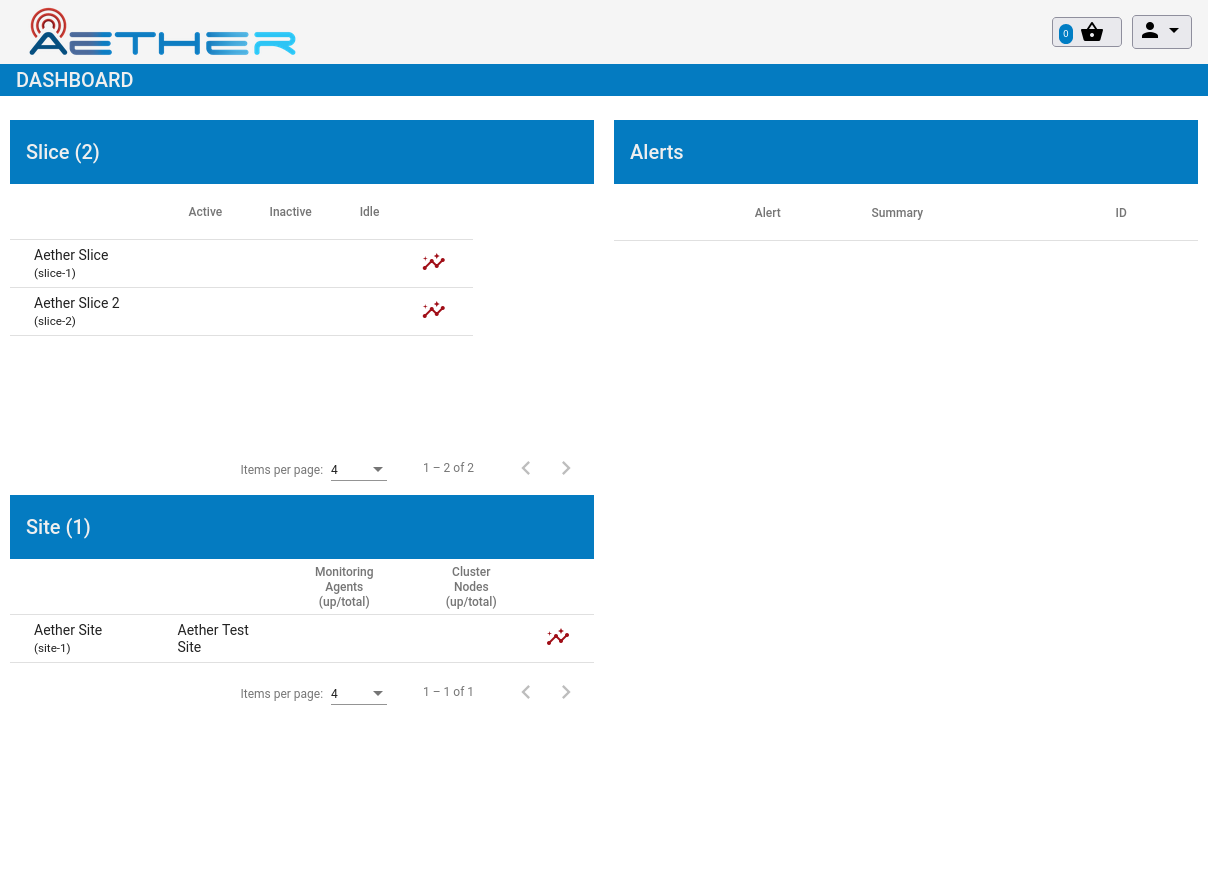
\includegraphics[width=0.8\textwidth]{Hassan_Thesis/images/LAB PC/Deployment&Netwroking/Aether.png}
        \caption{ROC Dashboard along with k8s running pods.}
        \label{fig:roc_dashboard}
    \end{figure}
    
Figure~\ref{fig:roc_dashboard} shows the Aether ROC (Runtime Operational Controller) dashboard, accessible after a successful full deployment. As illustrated, two network slices—\texttt{Aether Slice} and \texttt{Slice 2}—have been configured and are both associated with a single site named \texttt{Aether Site}. These slices correspond to two deployed UPF instances.The terminal output at the top confirms that the ROC system is active and fully deployed in the \texttt{aether-roc} namespace. It includes critical components such as \texttt{onos-config}, \texttt{onos-topo}, and \texttt{onos-cli}, which manage network state and configuration. The \texttt{roc-aether-roc-api} and \texttt{roc-aether-roc-gui} pods provide REST APIs and GUI access, while the \texttt{roc-consensus} pods form a distributed control layer for high availability. Monitoring and export capabilities are enabled through \texttt{roc-grafana} and \texttt{aether-mock-exporter}, ensuring observability across the ROC stack. The presence of the \texttt{roc-sdcore-adapter} bridges the ROC with the SD-Core platform.

    \item \textbf{Deployment of Additional UPF Instances:}  
    Additional UPF instances were deployed to enable multi-path routing and load balancing. Their configurations were set to harmonize with the SD-Core and reflect changes made via ROC.  
    % Insert screenshot showing multiple UPF instances in the deployment status
    \begin{figure}[H]
        \centering
        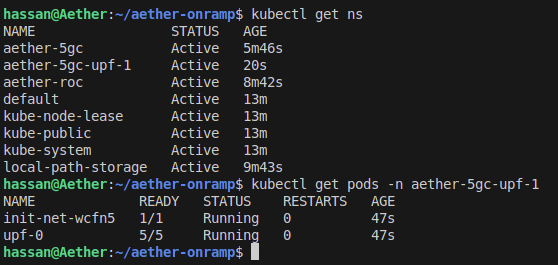
\includegraphics[width=0.8\textwidth]{Hassan_Thesis/images/LAB PC/Deployment&Netwroking/additionalupfadded.png}
        \caption{additional UPF instance in the \texttt{aether-5gc-upf-1} namespace.}
        \label{fig:multiple_upf}
    \end{figure}

In the Full Aether deployment, the default UPF is deployed in the \texttt{aether-5gc} namespace alongside the core network functions. To support multiple UPFs, an additional instance is deployed in a separate namespace named \texttt{aether-5gc-upf-1}. This approach allows for modular scaling and easier management of user plane functions. Figure~\ref{fig:multiple_upf} displays the active UPF pod (\texttt{upf-0}) running within the additional namespace, confirming a successful multi-UPF setup.

    \item \textbf{UERANSIM Deployment:}  
    The UERANSIM VM was configured with a single host-only network adapter (static IP \texttt{192.168.56.20}) to ensure isolation from direct internet access. This setup guarantees that all UE and gNodeB interactions are contained within the testbed and rely on the Aether VM for any external connectivity.

    \begin{figure}[H]
        \centering
        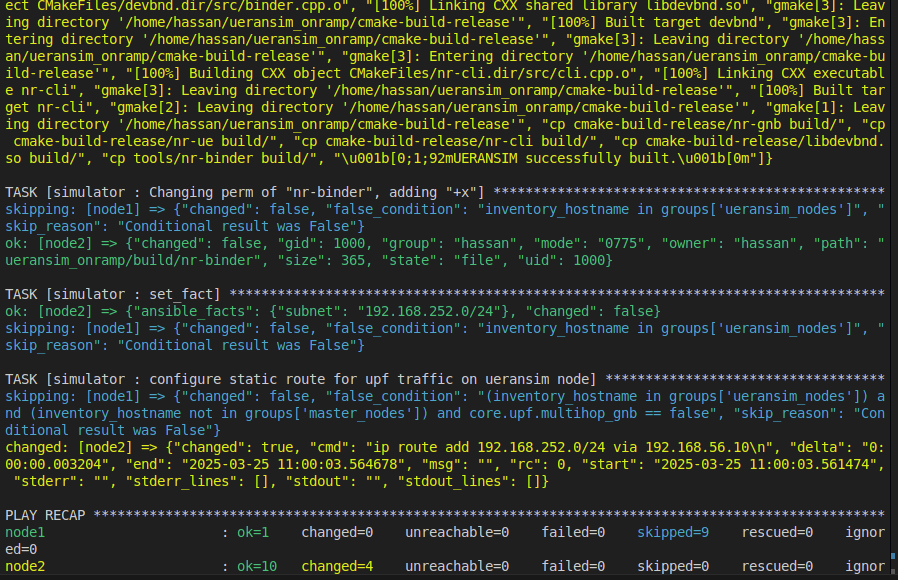
\includegraphics[width=0.8\textwidth]{Hassan_Thesis/images/LAB PC/Deployment&Netwroking/ueransiminstalled.png}
        \caption{UERANSIM Successfull Deployment.}
        \label{fig:ueransim_status}
    \end{figure}

    \item \textbf{Deployment of Aether Monitor:}  
    Aether Monitor was deployed alongside the core network services. Prometheus was configured to collect metrics from the SD-Core components and UPF instances, while Grafana was set up to provide a real-time dashboard for visualizing these metrics. This monitoring framework is essential for performance analysis and troubleshooting.
    \begin{figure}[H]
        \centering
        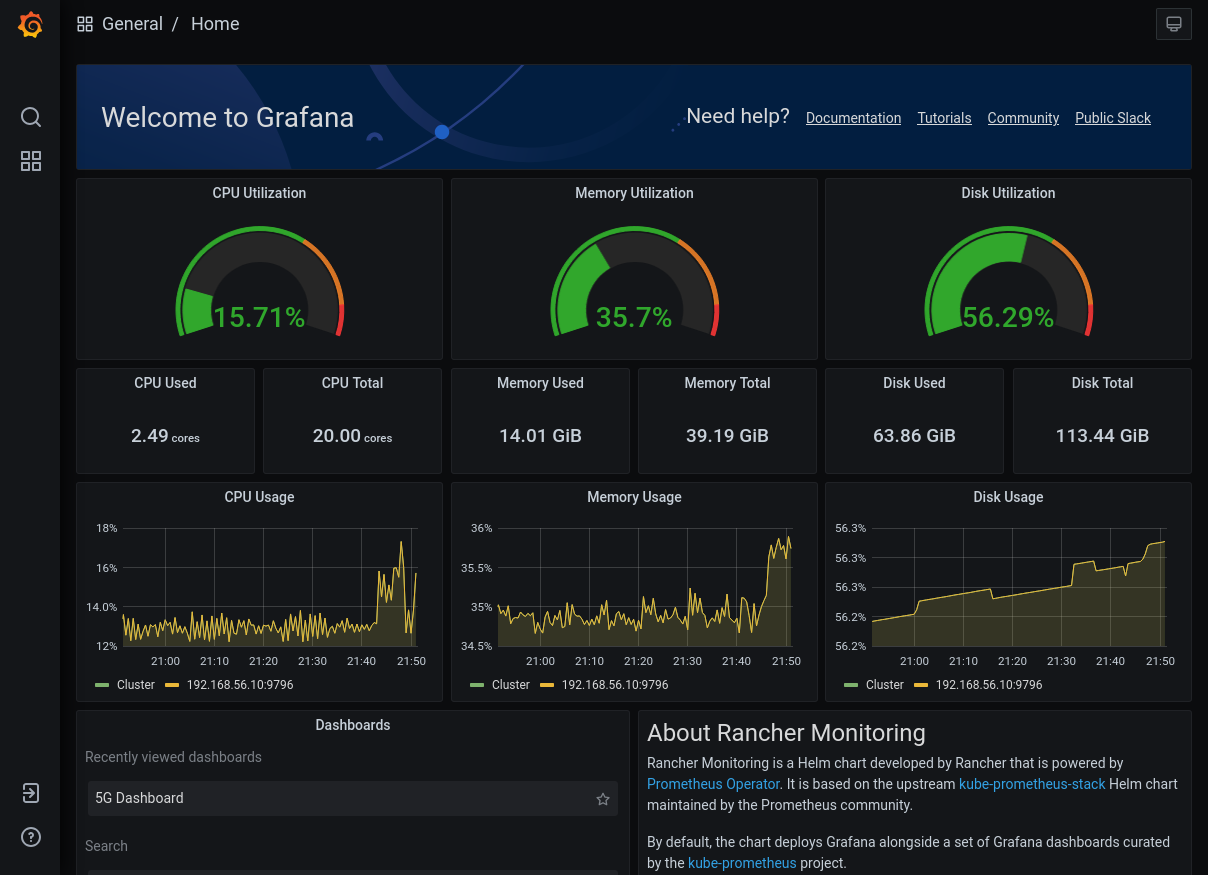
\includegraphics[width=0.8\textwidth]{Hassan_Thesis/images/LAB PC/Deployment&Netwroking/Home - Grafana.png}
        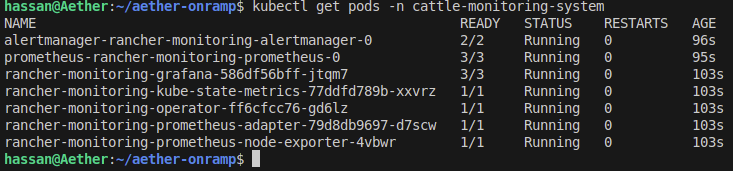
\includegraphics[width=0.8\textwidth]{Hassan_Thesis/images/LAB PC/Deployment&Netwroking/aethermoniterinstalled.png}
        \caption{Grafana Dashboard: Real-time visualization of network performance metrics.}
        \label{fig:grafana_dashboard}
    \end{figure}
\end{enumerate}

 The terminal output ~\ref{fig:grafana_dashboard} confirms that all monitoring-related pods (Prometheus, Grafana, Alertmanager, etc.) are running within the \texttt{cattle-monitoring-system} namespace, enabling real-time visualization and alerting for the Aether platform.

\subsection{Identified Issues and Platform Contributions}
\label{subsubsec:issues-solutions}

During the course of deployment and testing on the Lab PC, several issues were identified in the Aether platform that limited scalability and operational efficiency. Addressing these issues not only ensured the success of our own deployment but also resulted in meaningful contributions to the upstream codebase. Two key contributions were made: (1) improving IP address export for Prometheus, and (2) enhancing the dynamic handling of UPF routing and NAT configuration.

\paragraph{1. Exporting IP Address Metrics Directly from \texttt{metricfunc}}  
Initially, the Grafana dashboard retrieved the IP address of user equipment through the \texttt{smf-monitor} service. This dependency introduced complexity and made the monitoring pipeline less robust. To simplify the system and improve reliability, the IP address export functionality was integrated directly into the \texttt{metricfunc} module. This eliminated the need for the \texttt{smf-monitor} component, reducing overhead and potential points of failure.

The implemented changes were submitted as a Pull Request to the official Aether \texttt{metricfunc} repository and subsequently merged. A related update to the Grafana dashboard within the Aether AMP project removed the \texttt{smf-monitor} dependency entirely.

\begin{itemize}
    \item \textbf{Repository:} \texttt{omec-project/metricfunc}
    \item \textbf{Pull Request:} \href{https://github.com/omec-project/metricfunc/pull/127}{\#127}
    \item \textbf{Impact:} More efficient and reliable export of IP metrics for monitoring via Prometheus and Grafana.
\end{itemize}

\begin{itemize}
    \item \textbf{Repository:} \texttt{opennetworkinglab/aether-amp}
    \item \textbf{Pull Request:} \href{https://github.com/opennetworkinglab/aether-amp/pull/23}{\#23}
    \item \textbf{Impact:} Removal of \texttt{smf-monitor} dependency and simplification of dashboard configuration.
\end{itemize}

\paragraph{2. Dynamic UPF Routing and NAT Configuration Enhancements}  
The original deployment mechanism relied on a static \texttt{aether-ue-nat.service} configuration for NAT, which proved to be a limiting factor during scalability testing. When multiple UPFs were added, the static configuration required manual modifications and often resulted in errors such as \texttt{RTNETLINK answers: File exists} due to conflicting or duplicated routes.

To resolve this, a dynamic approach was introduced:
\begin{itemize}\raggedright
    \item The static NAT service file was replaced with a templated version (\texttt{aether-ue-nat.service.j2}) using Jinja2.
    \item The \texttt{install.yaml} task was updated to generate the NAT service dynamically based on the active UPF configuration.
    \item Routing logic was moved from the UPF role to the router role to better reflect separation of responsibilities.
    \item Logic was introduced to prevent duplicate route errors by checking for the existence of routes before adding them.
\end{itemize}

\textbf{Motivation and Benefits:}
\begin{itemize}
    \item Automatically adapts NAT configuration to reflect the current UPF topology.
    \item Eliminates the need for manual updates when deploying additional UPF instances.
    \item Ensures clean and error-free route management, facilitating seamless scalability.
\end{itemize}

\textbf{Testing and Validation:}
\begin{itemize}
    \item Successfully deployed Aether 5GC with multiple UPFs using the new dynamic approach.
    \item Verified dynamic generation of the NAT service and correctness of routing entries.
    \item Ensured no route duplication errors occurred during the addition of new UPFs.
\end{itemize}

\textbf{Status:} The proposed enhancements have been submitted to the upstream Aether platform as a pull request and are currently under review:
\begin{itemize}
    \item \textbf{Pull Request:} \href{https://github.com/opennetworkinglab/aether-5gc/pull/38}{\#38 –Enhancement: Dynamic UPF Routing and NAT Handling}
    \item \textbf{Review Status:} Pending (as of March 2025)
\end{itemize}

\medskip

These contributions not only streamlined our own experimental workflow but also addressed broader limitations in the Aether platform’s scalability. By contributing back to the upstream repositories, this thesis work has improved the automation, flexibility, and maintainability of the Aether deployment process.


\subsection{Summary of the Full Aether Deployment}

The deployment of multiple blueprints on the Lab PC resulted in the establishment of a robust, scalable, and dynamically managed 5G core network testbed. Key outcomes of this implementation include:

\begin{itemize}
    \item \textbf{Dynamic Core Network Management:}  
    The integration of ROC with the SD-Core enabled real-time configuration of network slices, user profiles, and device groups. This allowed for on-the-fly attachment of UPFs to slices and enhanced operational flexibility.
    
    \item \textbf{Scalable and Resilient UPF Deployment:}  
    Additional UPF instances were deployed successfully to support complex routing scenarios and load balancing. Improvements to the routing and NAT configuration process ensured seamless scalability without manual intervention.
    
    \item \textbf{Isolated RAN Simulation:}  
    The UERANSIM VM, operating within a host-only network and isolated from the internet, ensured that all UE and gNodeB simulations occurred entirely within a controlled lab environment, preserving experimental integrity.
    
    \item \textbf{Comprehensive Monitoring and Visualization:}  
    Aether Monitor was deployed to capture detailed performance metrics using Prometheus and visualize them via Grafana dashboards. Custom enhancements to metric collection simplified the architecture by removing redundant services and exposing essential metrics more directly.
    
    \item \textbf{Platform Enhancements and Contributions:}  
    Several issues encountered during the deployment process were addressed through custom improvements. Notably, IP address export was integrated directly into the metric function, eliminating dependency on the \texttt{smf-monitor} service. In addition, the NAT and routing configurations for UPFs were redesigned using Jinja2 templates and dynamic logic, significantly improving automation and reliability. These contributions were submitted to the official codebase for broader adoption.
\end{itemize}

These results validate the advanced deployment methodology presented in the 
Methodology chapter and demonstrate the Aether platform’s capability to support 
dynamic runtime operations, scalable UPF configurations, and real-time monitoring 
within a realistic lab setup. For an in-depth look at the specific YAML configuration 
used in this Lab PC scenario, refer to Appendix~\ref{sec:labpc-config}. The deployment 
also served as a foundation for further experimentation, performance evaluation, and 
direct contributions to the open-source ecosystem, as elaborated in the following chapters.

